% REE revelation deficit vs tau — posterior method v3, G=14, gamma=0.5
\documentclass[border=2mm]{standalone}
\usepackage{pgfplots}
\pgfplotsset{compat=1.18}
\definecolor{red}{rgb}{0.7, 0.11, 0.11}
\definecolor{blue}{rgb}{0.0, 0.20, 0.42}
\definecolor{green}{rgb}{0.11, 0.35, 0.02}
\begin{document}
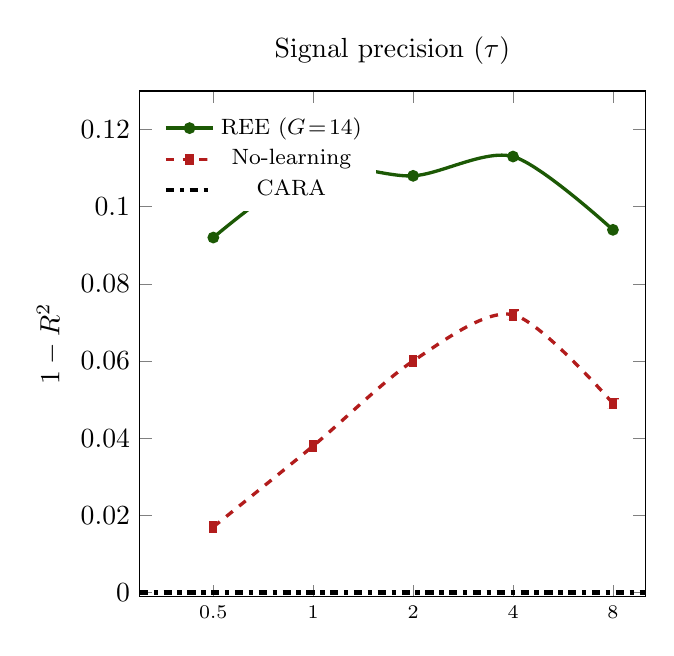
\begin{tikzpicture}
\begin{axis}[
  legend style={draw=none,legend pos=north west,font=\footnotesize},
  ticklabel style={/pgf/number format/fixed,/pgf/number format/precision=5},
  scaled ticks=false,
  ymin=-0.001, ymax=0.13, ylabel={$1-R^2$},
  xmin=0.3, xmax=10, xmode=log,
  xlabel={},
  xtick={0.5,1,2,4,8},
  xticklabels={0.5,1,2,4,8},
  xticklabel style={/pgf/number format/1000 sep=,font=\scriptsize},
  width=8cm, height=8cm,
  title={Signal precision ($\tau$)}]

% REE (posterior method v3, strict)
\addplot[very thick,color=green,smooth,mark=*,mark size=1.5pt]
  coordinates {
  (0.5,0.092)(1.0,0.110)(2.0,0.108)(4.0,0.113)(8.0,0.094)};

% No-learning (G=10, gamma=0.5)
\addplot[very thick,color=red,dashed,smooth,mark=square*,mark size=1.5pt]
  coordinates {
  (0.5,0.017)(1.0,0.038)(2.0,0.060)(4.0,0.072)(8.0,0.049)};

% CARA baseline
\addplot[ultra thick,color=black,dashdotted]
  coordinates {(0.3,0)(10,0)};

\legend{REE ($G\!=\!14$), No-learning, CARA}

\end{axis}
\end{tikzpicture}
\end{document}
